\documentclass[a4paper,11pt,exos]{nsi} % COMPILE WITH DRAFT


\pagestyle{empty}
\begin{document}

%Exercice 1E12


%\subsection*{NOM, Prénom : \dotfill} 

\classe{\premiere spé}
\titre{Ceinture marron 03 - Corrigé}
\maketitle\

\begin{exercice}[ : Trouver l'équation d'une parabole]
  Quelle est l'expression de la fonction polynomiale $f$ du second degré qui passe par les points de coordonnées $(-5;-121)$, $(0;9)$ et $(5;-61)$ ?\\
    Donner la forme développée de $f$.




      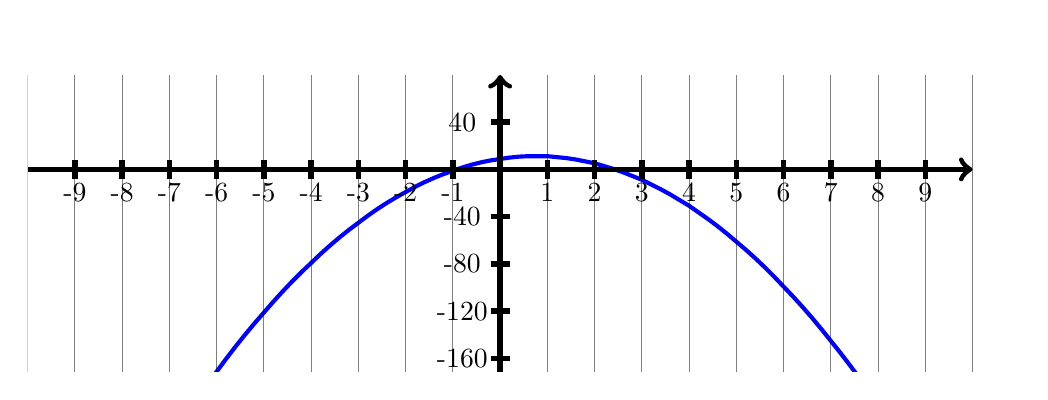
\begin{tikzpicture}[baseline,scale = 0.6]
      
          \tikzset{
            point/.style={
              thick,
              draw,
              cross out,
              inner sep=0pt,
              minimum width=5pt,
              minimum height=5pt,
            },
          }
          \clip (-10,-4.275) rectangle (11,3);
            
        \draw[color={blue},line width = 1.5] ;
        \draw[color={blue},line width = 1.5] ;
        \draw[color={blue},line width = 1.5] ;
        \draw[color={blue},line width = 1.5] ;
        \draw[color={blue},line width = 1.5] ;
        \draw[color={blue},line width = 1.5] ;
        \draw[color={blue},line width = 1.5] ;
        \draw[color={blue},line width = 1.5] ;
        \draw[color={blue},line width = 1.5] ;
        \draw[color={blue},line width = 1.5] ;
        \draw[color={blue},line width = 1.5] ;
        \draw[color={blue},line width = 1.5] ;
        \draw[color={blue},line width = 1.5] ;
        \draw[color={blue},line width = 1.5] ;
        \draw[color={blue},line width = 1.5] ;
        \draw[color={blue},line width = 1.5] (-7,-5.73)--(-6.8,-5.42)--(-6.6,-5.12)--(-6.4,-4.83)--(-6.2,-4.55)--(-6,-4.28)--(-5.8,-4.01)--(-5.6,-3.75)--(-5.4,-3.5)--(-5.2,-3.26)--(-5,-3.03)--(-4.8,-2.8)--(-4.6,-2.58)--(-4.4,-2.37)--(-4.2,-2.17)--(-4,-1.98)--(-3.8,-1.79)--(-3.6,-1.61)--(-3.4,-1.44)--(-3.2,-1.28)--(-3,-1.13)--(-2.8,-0.98)--(-2.6,-0.84)--(-2.4,-0.71)--(-2.2,-0.59)--(-2,-0.48)--(-1.8,-0.37)--(-1.6,-0.27)--(-1.4,-0.18)--(-1.2,-0.1)--(-1,-0.03)--(-0.8,0.04)--(-0.6,0.1)--(-0.4,0.15)--(-0.2,0.19)--(0,0.22)--(0.2,0.25)--(0.4,0.27)--(0.6,0.28)--(0.8,0.28)--(1,0.28)--(1.2,0.26)--(1.4,0.24)--(1.6,0.21)--(1.8,0.17)--(2,0.13)--(2.2,0.07)--(2.4,0.01)--(2.6,-0.06)--(2.8,-0.14)--(3,-0.22)--(3.2,-0.32)--(3.4,-0.42)--(3.6,-0.53)--(3.8,-0.65)--(4,-0.77)--(4.2,-0.91)--(4.4,-1.05)--(4.6,-1.2)--(4.8,-1.36)--(5,-1.53)--(5.2,-1.7)--(5.4,-1.88)--(5.6,-2.07)--(5.8,-2.27)--(6,-2.48)--(6.2,-2.69)--(6.4,-2.91)--(6.6,-3.14)--(6.8,-3.38)--(7,-3.63)--(7.2,-3.88)--(7.4,-4.14)--(7.6,-4.41)--(7.8,-4.69)--(8,-4.98)--(8.2,-5.27)--(8.4,-5.57)--(8.6,-5.88);
        \draw[color={blue},line width = 1.5] ;
        \draw[color={blue},line width = 1.5] ;
        \draw[color={blue},line width = 1.5] ;
        \draw[color={blue},line width = 1.5] ;
        \draw[color={blue},line width = 1.5] ;
        \draw[color={blue},line width = 1.5] ;
        \draw[color={blue},line width = 1.5] ;
        
        \draw[color ={black},line width = 2,->] (-10,0)--(10,0);
        \draw[color ={black},line width = 2,->] (0,-6)--(0,2);
        \draw[color ={black},opacity = 0.5] (1,-6)--(1,2);
        \draw[color ={black},opacity = 0.5] (2,-6)--(2,2);
        \draw[color ={black},opacity = 0.5] (3,-6)--(3,2);
        \draw[color ={black},opacity = 0.5] (4,-6)--(4,2);
        \draw[color ={black},opacity = 0.5] (5,-6)--(5,2);
        \draw[color ={black},opacity = 0.5] (6,-6)--(6,2);
        \draw[color ={black},opacity = 0.5] (7,-6)--(7,2);
        \draw[color ={black},opacity = 0.5] (8,-6)--(8,2);
        \draw[color ={black},opacity = 0.5] (9,-6)--(9,2);
        \draw[color ={black},opacity = 0.5] (10,-6)--(10,2);
        \draw[color ={black},opacity = 0.5] (-1,-6)--(-1,2);
        \draw[color ={black},opacity = 0.5] (-2,-6)--(-2,2);
        \draw[color ={black},opacity = 0.5] (-3,-6)--(-3,2);
        \draw[color ={black},opacity = 0.5] (-4,-6)--(-4,2);
        \draw[color ={black},opacity = 0.5] (-5,-6)--(-5,2);
        \draw[color ={black},opacity = 0.5] (-6,-6)--(-6,2);
        \draw[color ={black},opacity = 0.5] (-7,-6)--(-7,2);
        \draw[color ={black},opacity = 0.5] (-8,-6)--(-8,2);
        \draw[color ={black},opacity = 0.5] (-9,-6)--(-9,2);
        \draw[color ={black},opacity = 0.5] (-10,-6)--(-10,2);
        \draw[color ={black},line width = 2] (1,-0.2)--(1,0.2);
        \draw[color ={black},line width = 2] (2,-0.2)--(2,0.2);
        \draw[color ={black},line width = 2] (3,-0.2)--(3,0.2);
        \draw[color ={black},line width = 2] (4,-0.2)--(4,0.2);
        \draw[color ={black},line width = 2] (5,-0.2)--(5,0.2);
        \draw[color ={black},line width = 2] (6,-0.2)--(6,0.2);
        \draw[color ={black},line width = 2] (7,-0.2)--(7,0.2);
        \draw[color ={black},line width = 2] (8,-0.2)--(8,0.2);
        \draw[color ={black},line width = 2] (9,-0.2)--(9,0.2);
        \draw[color ={black},line width = 2] (-1,-0.2)--(-1,0.2);
        \draw[color ={black},line width = 2] (-2,-0.2)--(-2,0.2);
        \draw[color ={black},line width = 2] (-3,-0.2)--(-3,0.2);
        \draw[color ={black},line width = 2] (-4,-0.2)--(-4,0.2);
        \draw[color ={black},line width = 2] (-5,-0.2)--(-5,0.2);
        \draw[color ={black},line width = 2] (-6,-0.2)--(-6,0.2);
        \draw[color ={black},line width = 2] (-7,-0.2)--(-7,0.2);
        \draw[color ={black},line width = 2] (-8,-0.2)--(-8,0.2);
        \draw[color ={black},line width = 2] (-9,-0.2)--(-9,0.2);
        \draw[color ={black},line width = 2] (-0.2,1)--(0.2,1);
        \draw[color ={black},line width = 2] (-0.2,-1)--(0.2,-1);
        \draw[color ={black},line width = 2] (-0.2,-2)--(0.2,-2);
        \draw[color ={black},line width = 2] (-0.2,-3)--(0.2,-3);
        \draw[color ={black},line width = 2] (-0.2,-4)--(0.2,-4);
        \draw[color ={black},line width = 2] (-0.2,-5)--(0.2,-5);
        \draw [color={black},fill opacity = 1] (1,-0.5) node[anchor = center,scale=1] {1};
        \draw [color={black},fill opacity = 1] (2,-0.5) node[anchor = center,scale=1] {2};
        \draw [color={black},fill opacity = 1] (3,-0.5) node[anchor = center,scale=1] {3};
        \draw [color={black},fill opacity = 1] (4,-0.5) node[anchor = center,scale=1] {4};
        \draw [color={black},fill opacity = 1] (5,-0.5) node[anchor = center,scale=1] {5};
        \draw [color={black},fill opacity = 1] (6,-0.5) node[anchor = center,scale=1] {6};
        \draw [color={black},fill opacity = 1] (7,-0.5) node[anchor = center,scale=1] {7};
        \draw [color={black},fill opacity = 1] (8,-0.5) node[anchor = center,scale=1] {8};
        \draw [color={black},fill opacity = 1] (9,-0.5) node[anchor = center,scale=1] {9};
        \draw [color={black},fill opacity = 1] (-1,-0.5) node[anchor = center,scale=1] {-1};
        \draw [color={black},fill opacity = 1] (-2,-0.5) node[anchor = center,scale=1] {-2};
        \draw [color={black},fill opacity = 1] (-3,-0.5) node[anchor = center,scale=1] {-3};
        \draw [color={black},fill opacity = 1] (-4,-0.5) node[anchor = center,scale=1] {-4};
        \draw [color={black},fill opacity = 1] (-5,-0.5) node[anchor = center,scale=1] {-5};
        \draw [color={black},fill opacity = 1] (-6,-0.5) node[anchor = center,scale=1] {-6};
        \draw [color={black},fill opacity = 1] (-7,-0.5) node[anchor = center,scale=1] {-7};
        \draw [color={black},fill opacity = 1] (-8,-0.5) node[anchor = center,scale=1] {-8};
        \draw [color={black},fill opacity = 1] (-9,-0.5) node[anchor = center,scale=1] {-9};
        \draw [color={black},fill opacity = 1] (-0.8,1) node[anchor = center,scale=1] {40};
        \draw [color={black},fill opacity = 1] (-0.8,-1) node[anchor = center,scale=1] {-40};
        \draw [color={black},fill opacity = 1] (-0.8,-2) node[anchor = center,scale=1] {-80};
        \draw [color={black},fill opacity = 1] (-0.8,-3) node[anchor = center,scale=1] {-120};
        \draw [color={black},fill opacity = 1] (-0.8,-4) node[anchor = center,scale=1] {-160};
        \draw [color={black},fill opacity = 1] (-0.8,-5) node[anchor = center,scale=1] {-200};
      
      \end{tikzpicture}\\
\end{exercice}

Soit $f(x)=ax^2+bx+c$ , l'expression de la fonction cherchée, comme $f(0)=9$ nous en déduisons que $c={\color{red}\boldsymbol{9}}$.\\Donc $f(x)=ax^2+bx{\color{red}\boldsymbol{+9}}$.\\En substituant dans cette expression les valeurs de l'énoncé, nous obtenons :\\$\begin{cases}
    -61=a\times5^2+b\times5+9=25a +5b +9 \\
    -121=a\times(-5)^2+b\times(-5)+9=25a -5b +9
     \end{cases}$\\Ce qui équivaut à \\$\begin{cases}
     -61-9=-70=25a +5b \\
     -121-9=-130=25a -5b
       \end{cases}$\\En ajoutant et en soustrayant les équations membre à membre, on obtient :\\
    $\begin{cases}
    -200=50a \\
    60=10b
     \end{cases}$\\La résolution de ce système donne $a={\color{blue}\boldsymbol{-4}}$ et $b={\color{green}\boldsymbol{6}}$.\\D'où $f(x)={\color{blue}\boldsymbol{-4}}x^2 {\color{green}\boldsymbol{+6}}x  {\color{red}\boldsymbol{+9}}$\\
    

\end{document}